\lstinputlisting[language=C++]{solutions/loop_unrolling/factor2/fir_loop_unrolling_manual_factor2.cpp}
\lstinputlisting[language=C++]{solutions/loop_unrolling/factor2/fir_loop_unrolling_automatic_factor2.cpp}
\lstinputlisting[language=C++]{solutions/loop_unrolling/factor2/fir_loop_unrolling_automatic_partiotioning_factor2.cpp}

\begin{table}[H]
    \centering
    \begin{tabular}{|c|c|c|c|c|}
        \hline
        \textbf{Solution} & \textbf{Clock} & \textbf{Target} & \textbf{Estimated} & \textbf{Uncertainty} \\
        \hline
        Manuale & ap\_clk & 10.00 & 8.510 & 1.25 \\
        \hline
        Automatico & ap\_clk & 10.00 & 8.510 & 1.25 \\
        \hline
        Automatico con Partitioning & ap\_clk & 10.00 & 8.510 & 1.25 \\
        \hline
    \end{tabular}
    \caption{HLS Loop Unrolling Factor=2 Solution Timing Summary (ns)}
    \label{tab:hls-loop-unrolling-factor2-solution-timing-summary}
\end{table}

Si può notare come la latenza associata alla soluzione hardware basata su unrolling manuale sia la medesima di quella basata su unrolling automatico (effettuato mediante pragma). Questo è dovuto al fatto che l'implementazione è la stessa: nel primo caso è effettuato manualmente mentre nel secondo caso è effettuato mediante direttiva proprietaria del tool. Invece, nel caso della soluzione hardware basata su unrolling automatico e partitioning, si riscontra una latenza maggiore. Questo risultato è dovuto al fatto che, tramite il pragma di partizionamento, si è dovuto gestire, inoltre, letture e scritture in parallelo.

\begin{table}[H]
    \centering
    \begin{tabular}{|c|c|c|c|c|}
        \hline
        \multicolumn{1}{|c|}{\textbf{Solution}} & \multicolumn{2}{|c|}{\textbf{Latency}} & \multicolumn{2}{|c|}{\textbf{Interval}} \\
        & min & max & min & max \\
        \hline
        Manuale & 56 & 56 & 56 & 56 \\
        \hline
        Automatico & 56 & 56 & 56 & 56 \\
        \hline
        Automatico con Partitioning & 61 & 66 & 61 & 66 \\
        \hline
    \end{tabular}
    \caption{HLS Loop Unrolling Factor=2 Solution Latency Summary (clock cycles)}
    \label{tab:hls-loop-unrolling-factor2-solution-latency-summary}
\end{table}

Si può evidenziare come, nel caso della soluzione hardware con urolling automatico e partizionamento, l'aumento della latenza si ha soltanto in corrispondenza del loop di shifting, cioè proprio dove è stato collocato il pragma di partitioning.

\begin{table}[H]
    \centering
    \begin{tabular}{|c|c|c|c|c|c|c|c|c|c|}
        \hline
        \multicolumn{1}{|c|}{\textbf{Solution}} & \multicolumn{1}{|c|}{Loop Name} & \multicolumn{2}{|c|}{\textbf{Latency}} & \multicolumn{2}{c|}{\textbf{Iteration Latency}} & \multicolumn{2}{c|}{\textbf{Initiation Interval}} & \multicolumn{1}{c|}{\textbf{Trip}}  \\
        &  & min & max & min & max & achieved & target & \textbf{Count} \\
        \hline
        Manuale & - loopShifting & 10 & 10 & 2 & 2 & - & - & 5 \\
        & - loopAccumulator & 44 & 44 & 4 & 4 & - & - & 11 \\
        \hline
        Automatico & - loopShifting & 10 & 10 & 2 & 2 & - & - & 5 \\
        & - loopAccumulator & 44 & 44 & 4 & 4 & - & - & 11 \\
        \hline
        Automatico  & - loopShifting & 15 & 20 & 3 & 4 & - & - & 5 \\
        con Partitioning & - loopAccumulator & 44 & 44 & 4 & 4 & - & - & 11 \\
        \hline
    \end{tabular}
    \caption{HLS Loop Unrolling Factor=2 Solution Latency Loops Summary }
    \label{tab:hls-loop-unrolling-factor2-solution-loop-summary}
\end{table}

Aprendo la sezione Analysis del tool si può vedere meglio nel dettaglio che, all'interno del loop di shifting, sono presenti 2 shifting in parallelo (dal momento che è stato considerato un fattore di parallelismo pari a 2) sia peer la soluzione hardware di unrolling manuale sia per quella di unrolling automatico (mediante pragma).

\begin{figure}[H]
    \centering
    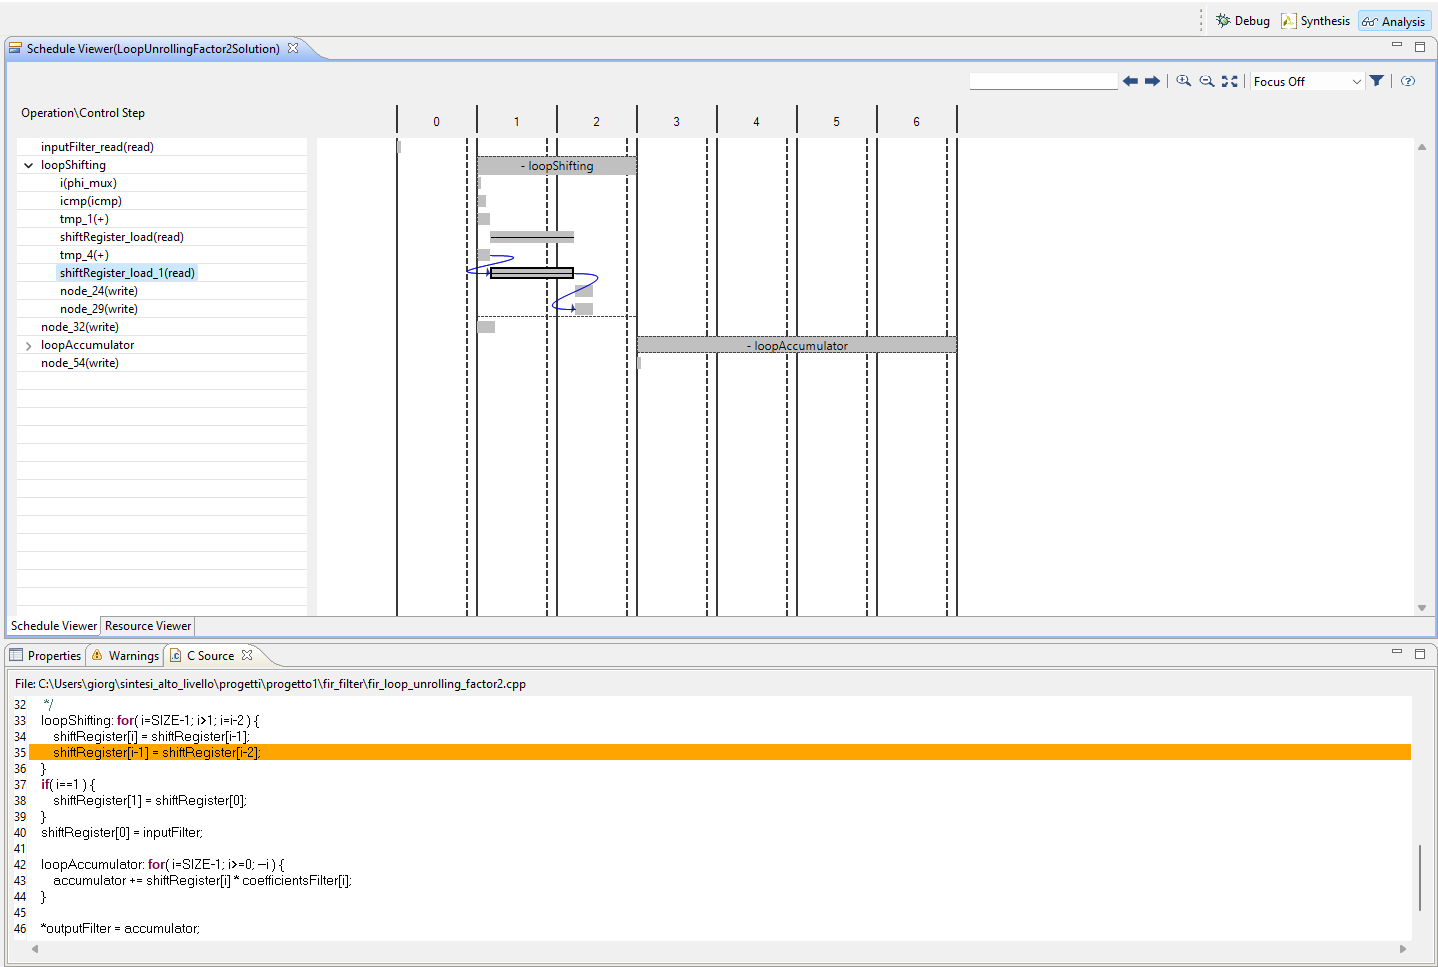
\includegraphics[width=0.9\textwidth]{solutions/loop_unrolling/factor2/loopunrollingmanual2.png}
    \caption{HLS Loop Unrolling Manual Factor=2 Analysis}
\end{figure}

\begin{figure}[H]
    \centering
    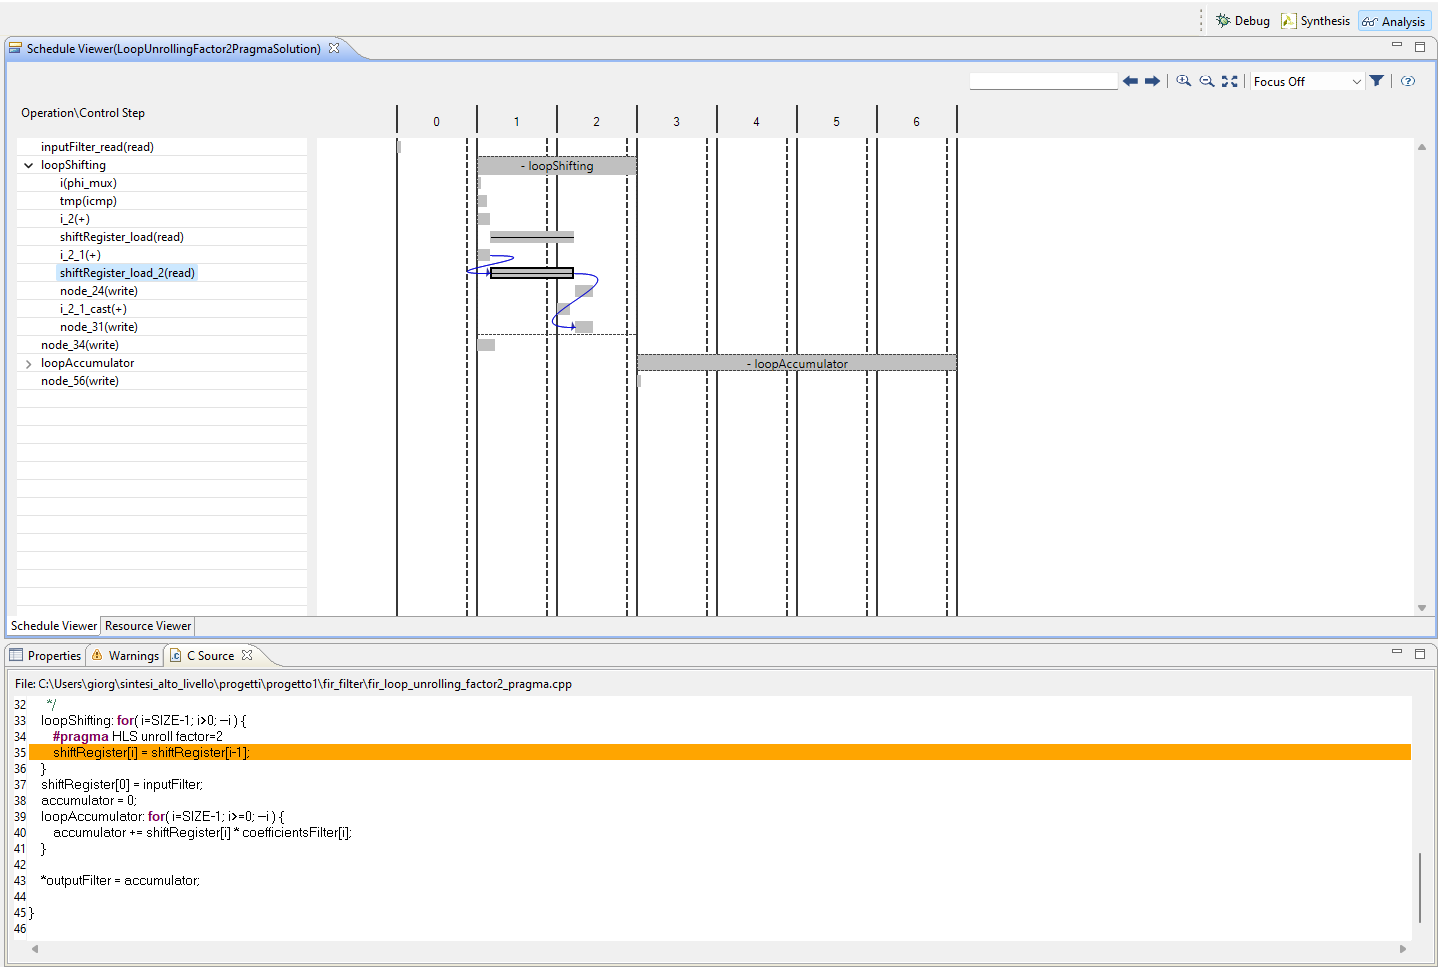
\includegraphics[width=0.9\textwidth]{solutions/loop_unrolling/factor2/loopunrollingautomatic2.png}
    \caption{HLS Loop Unrolling Automatic Factor=2 Analysis}
\end{figure}

Analizzando nel dettaglio il report si può notare come il numero di DSP e LUT sia pressocché il medesimo per tutte e tre le soluzioni hardware proposte. Per quanto riguarda, invece, il numero di BRAM utilizzate, le soluzioni basate su unrolling manuale e automatico presentano un'utilizzazione pari a 2, mentre quella basta su unrolling automatico e partitioning presenta un numero di BRAM utilizzato pari a 0. Questo è dovuto al fatto che il pragma di partizionamento, al fine di garantire accessi di read/write in memoria in parallelo, impone di non utilizzare le BRAM dual-port (che limiterebbero tali accessi). In particolare, impostando la tipologia di partizionamento \textit{complete}, la direttiva fa in modo che la soluzione hardware impieghi come memoria dei singoli registri, cosí che siano garantiti gli accessi in memoria in parallelo. Tanto è vero che si può notare un aumento considerevole dei FF in corrispondenza dell'architettura basata su unrolling automatico e partizionamento.

\begin{table}[H]
    \centering
    \begin{tabular}{|c|c|c|c|c|}
        \hline
        \textbf{Solution} & \textbf{BRAM\_18K} & \textbf{DSP48E} & \textbf{FF} & \textbf{LUT} \\
        \hline
        Manuale & 2 & 2 & 145 & 236 \\
        \hline
        Automatico & 2 & 2 & 141 & 251 \\
        \hline
        Automatico con Partitioning & 0 & 2 & 912 & 289 \\
        \hline
    \end{tabular}
    \caption{HLS Loop Unrolling Factor=2 Solution Utilization Estimates [\#]}
    \label{tab:hls-loop-unrolling-factor2-solution-utilization-report}
\end{table}

Qui di seguito vengono riportati i report relativi alla C/RTL Cosimulation, dove è possibile analizzare il numero di cicli di clock che servono per ottenere un risultato in uscita, e quello relativo a Export RTL.

\begin{table}[H]
    \centering
    \begin{tabular}{|c|c|c|c|c|c|c|c|c|}
        \hline
        \multicolumn{1}{|c|}{\textbf{Solution}} & \multicolumn{1}{|c|}{RTL} & \multicolumn{1}{|c|}{Status} & \multicolumn{3}{c|}{\textbf{Latency}} & \multicolumn{3}{c|}{\textbf{Interval}} \\
        & &  & min & avg & max & min & avg & max \\
        \hline
        Manuale & VHDL & Pass & 56 & 56 & 57 & 56 & 56 & 57 \\
        \hline
        Automatico & VHDL & Pass & 56 & 56 & 57 & 56 & 56 & 57 \\
        \hline
        Automatico con Partitioning & VHDL & Pass & 65 & 65 & 66 & 65 & 65 & 66 \\
        \hline
    \end{tabular}
    \caption{HLS Loop Unrolling Factor=2 Solution C/RTL Cosimulation Report }
    \label{tab:hls-loop-unrolling-factor2-solution-cosimulation-report}
\end{table}

\begin{table}[H]
    \centering
    \begin{tabular}{|c|c|c|c|c|c|c|c|c|}
        \hline
        \textbf{Solution} & \textbf{SLICE} & \textbf{LUT} & \textbf{FF} & \textbf{DSP} & \textbf{BRAM} & \textbf{CP} & \textbf{CP} & \textbf{CP} \\
        & & & & & & \textbf{required} & \textbf{achieved} & \textbf{achieved}\\
        & & & & & & & \textbf{post-} & \textbf{post-}\\
        & & & & & & & \textbf{synthesis} & \textbf{implementation}\\
        \hline
        Manuale & 31 & 97 & 72 & 2 & 2 & 10 & 5.745 & 5.692 \\
        \hline
        Automatico & 29 & 97 & 72 & 2 & 2 & 10 & 5.745 & 5.692 \\
        \hline
        Automatico  & 294 & 413 & 843 & 2 & 0 & 10 & 5.745 & 6.188 \\
        con Partitioning & & & & & & & & \\
        \hline
    \end{tabular}
    \caption{HLS Loop Unrolling Factor=2 Solution Export RTL Report}
    \label{tab:vivado-loop-unrolling-factor2-solution-export-rtl-report}
\end{table}


Pertanto, importando l'IP in Vivado e impostando un clock constraint pari a 10ns è possibile analizzare i seguenti report di risorse, timing, potenza dinamica ed energia per singola operazione.
\lstinputlisting[language=VHDL]{solutions/loop_unrolling/factor2/clk_constraint.xdc}

Analizzando il report di utilizzazione delle risorse generato da Vivado dopo aver effettuato il processo di implementazione, è possibile notare come il numero di risorse stimato dal tool HLS è leggermente mutato. Però, si può evidenziare come il cambiamento delle risorse tra le varie soluzioni hardware è il medesimo, cioè il numero di LUT e FF nel caso dell'implementazione con unrolling automatico e partitioning sia aumentato considerevolmente e il numero di BRAM si è ridotto a zero.

\begin{table}[H]
    \centering
    \begin{tabular}{|c|c|c|c|c|c|c|c|}
        \hline
        \textbf{Solution} & \textbf{LUT} & \textbf{LUTRAM} & \textbf{FF} & \textbf{BRAM} & \textbf{DSP} & \textbf{IO} & \textbf{BUFG} \\
        \hline
        Manuale & 98 & 0 & 72 & 1 & 2 & 71 & 1 \\
        \hline
        Automatico & 98 & 0 & 72 & 1 & 2 & 71 & 1 \\
        \hline
        Automatico & 413 & 0 & 843 & 0 & 2 & 71 & 1 \\
        con Partitioning & & & & & & & \\
        \hline
    \end{tabular}
    \caption{Vivado Loop Unrolling Factor=2 Solution Utilization Report [\#]}
    \label{tab:vivado-loop-unrolling-factor2-utilization-report}
\end{table}

Si è, inoltre, analizzato l'utilizzazione delle risorse effettuando un confronto con la soluzione hardware basata sulla scissione del loop dal momento che tali architetture basate su unrolling sono basate sulla prima citata. In particolare, si può notare come il numero di risorse utilizzate sia pressoché il medesimo tra la soluzione hardware basta su loop fission e quelle basate rispettivamente sull'unrolling manuale e automatico di fattore 2. Più nello specifico, considerando le implementazioni basate sul parallelismo manuale e automatico rispetto a quella basta sul loop fission, il numero di LUT è diminuito di circa il $40\%$, il numero di FF è diminuito di circa il $32\%$ e il numero di BRAM è aumentato di un'unità. Invece, effettuando un confronto tra quella basata su partitioning e quella basata sulla scissione del loop, il numero di LUT è aumentato di circa il $161\%$ e il numero di FF di circa il $695\%$.

\begin{figure}[H]
    \centering
    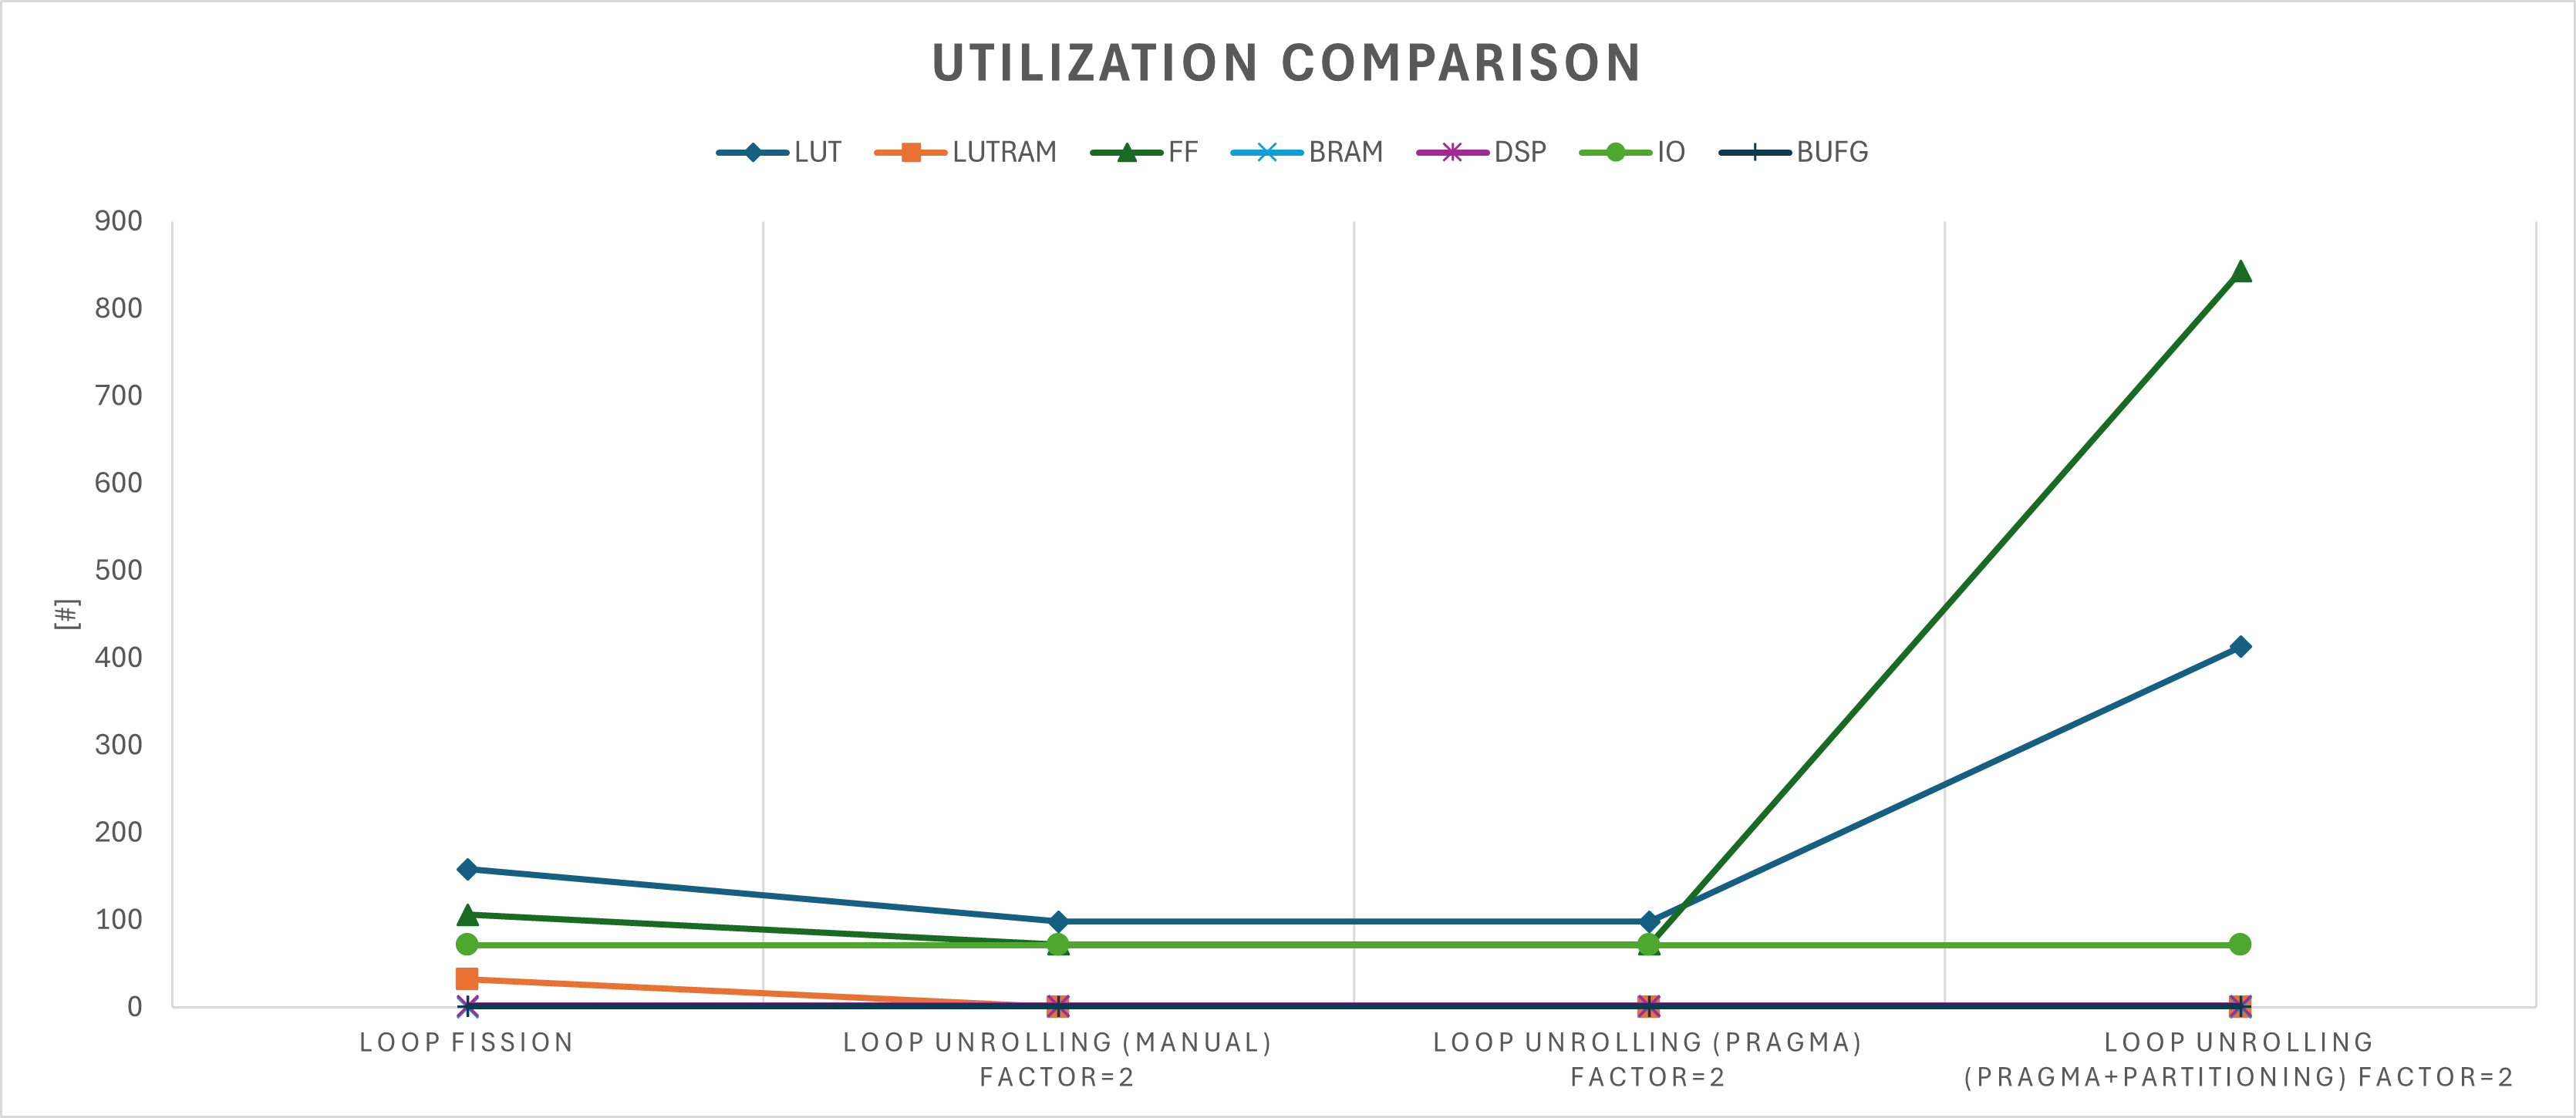
\includegraphics[width=0.9\textwidth]{solutions/loop_unrolling/factor2/loopunrollingfactor2utilization.png}
    \caption{Vivado Loop Unrolling Factor=2 Utilization Plot}
    \label{fig:vivado-loop-unrolling-factor2-utilization-plot}
\end{figure}

Infine, per quanto riguarda il timing, è possibile notare come il numero di cicli sia pressocché il medesimo tra la soluzione basata su unrolling manuale e quella basata su unrolling automatico. Invece, come precedentemente citato, la soluzione basata su partizionamento presenta un numero di cicli di clock, tali per garantire un risultato, maggiore.

\begin{table}[H]
    \centering
    \begin{tabular}{|c|c|c|c|c|}
        \hline
        \textbf{Solution} & \textbf{Cycles} [\#] & \textbf{Clock Constraint} [ns] & \textbf{WNS} [ns] & \textbf{Maximum Clock} \\
        & & & & \textbf{Frequency} [MHz] \\
        \hline
        Manuale & 57 & 10 & 4.33 & 176.366843 \\
        \hline
        Automatico & 57 & 10 & 4.33 & 176.366843 \\
        \hline
        Automatico & 66 & 10 & 3.469 & 153.1159087 \\
        con Partitioning & & & & \\
        \hline
    \end{tabular}
    \caption{Vivado Loop Unrolling Factor=2 Solution Timing Report}
    \label{tab:vivado-loop-unrolling-factor2-solution-timing-report}
\end{table}

Effettuando un confronto grafico e tenendo conto anche della soluzione basata sulla scissione del loop, è possibile evidenziare un numero di cicli di clock, tali per garantire un risultato, un WNS e una maximum clock frequency pressoché uguali tra l'implementazione basata su loop fission e quella basata su partizionamento. Questo accade dal momento che la soluzione hardware basata su unrolling automatico e partitioning fa diminuire il numero di cicli di clock tramite il parallelismo e lo fa aumentare allo stesso tempo a causa del partizionamento. 

\begin{figure}[H]
    \centering
    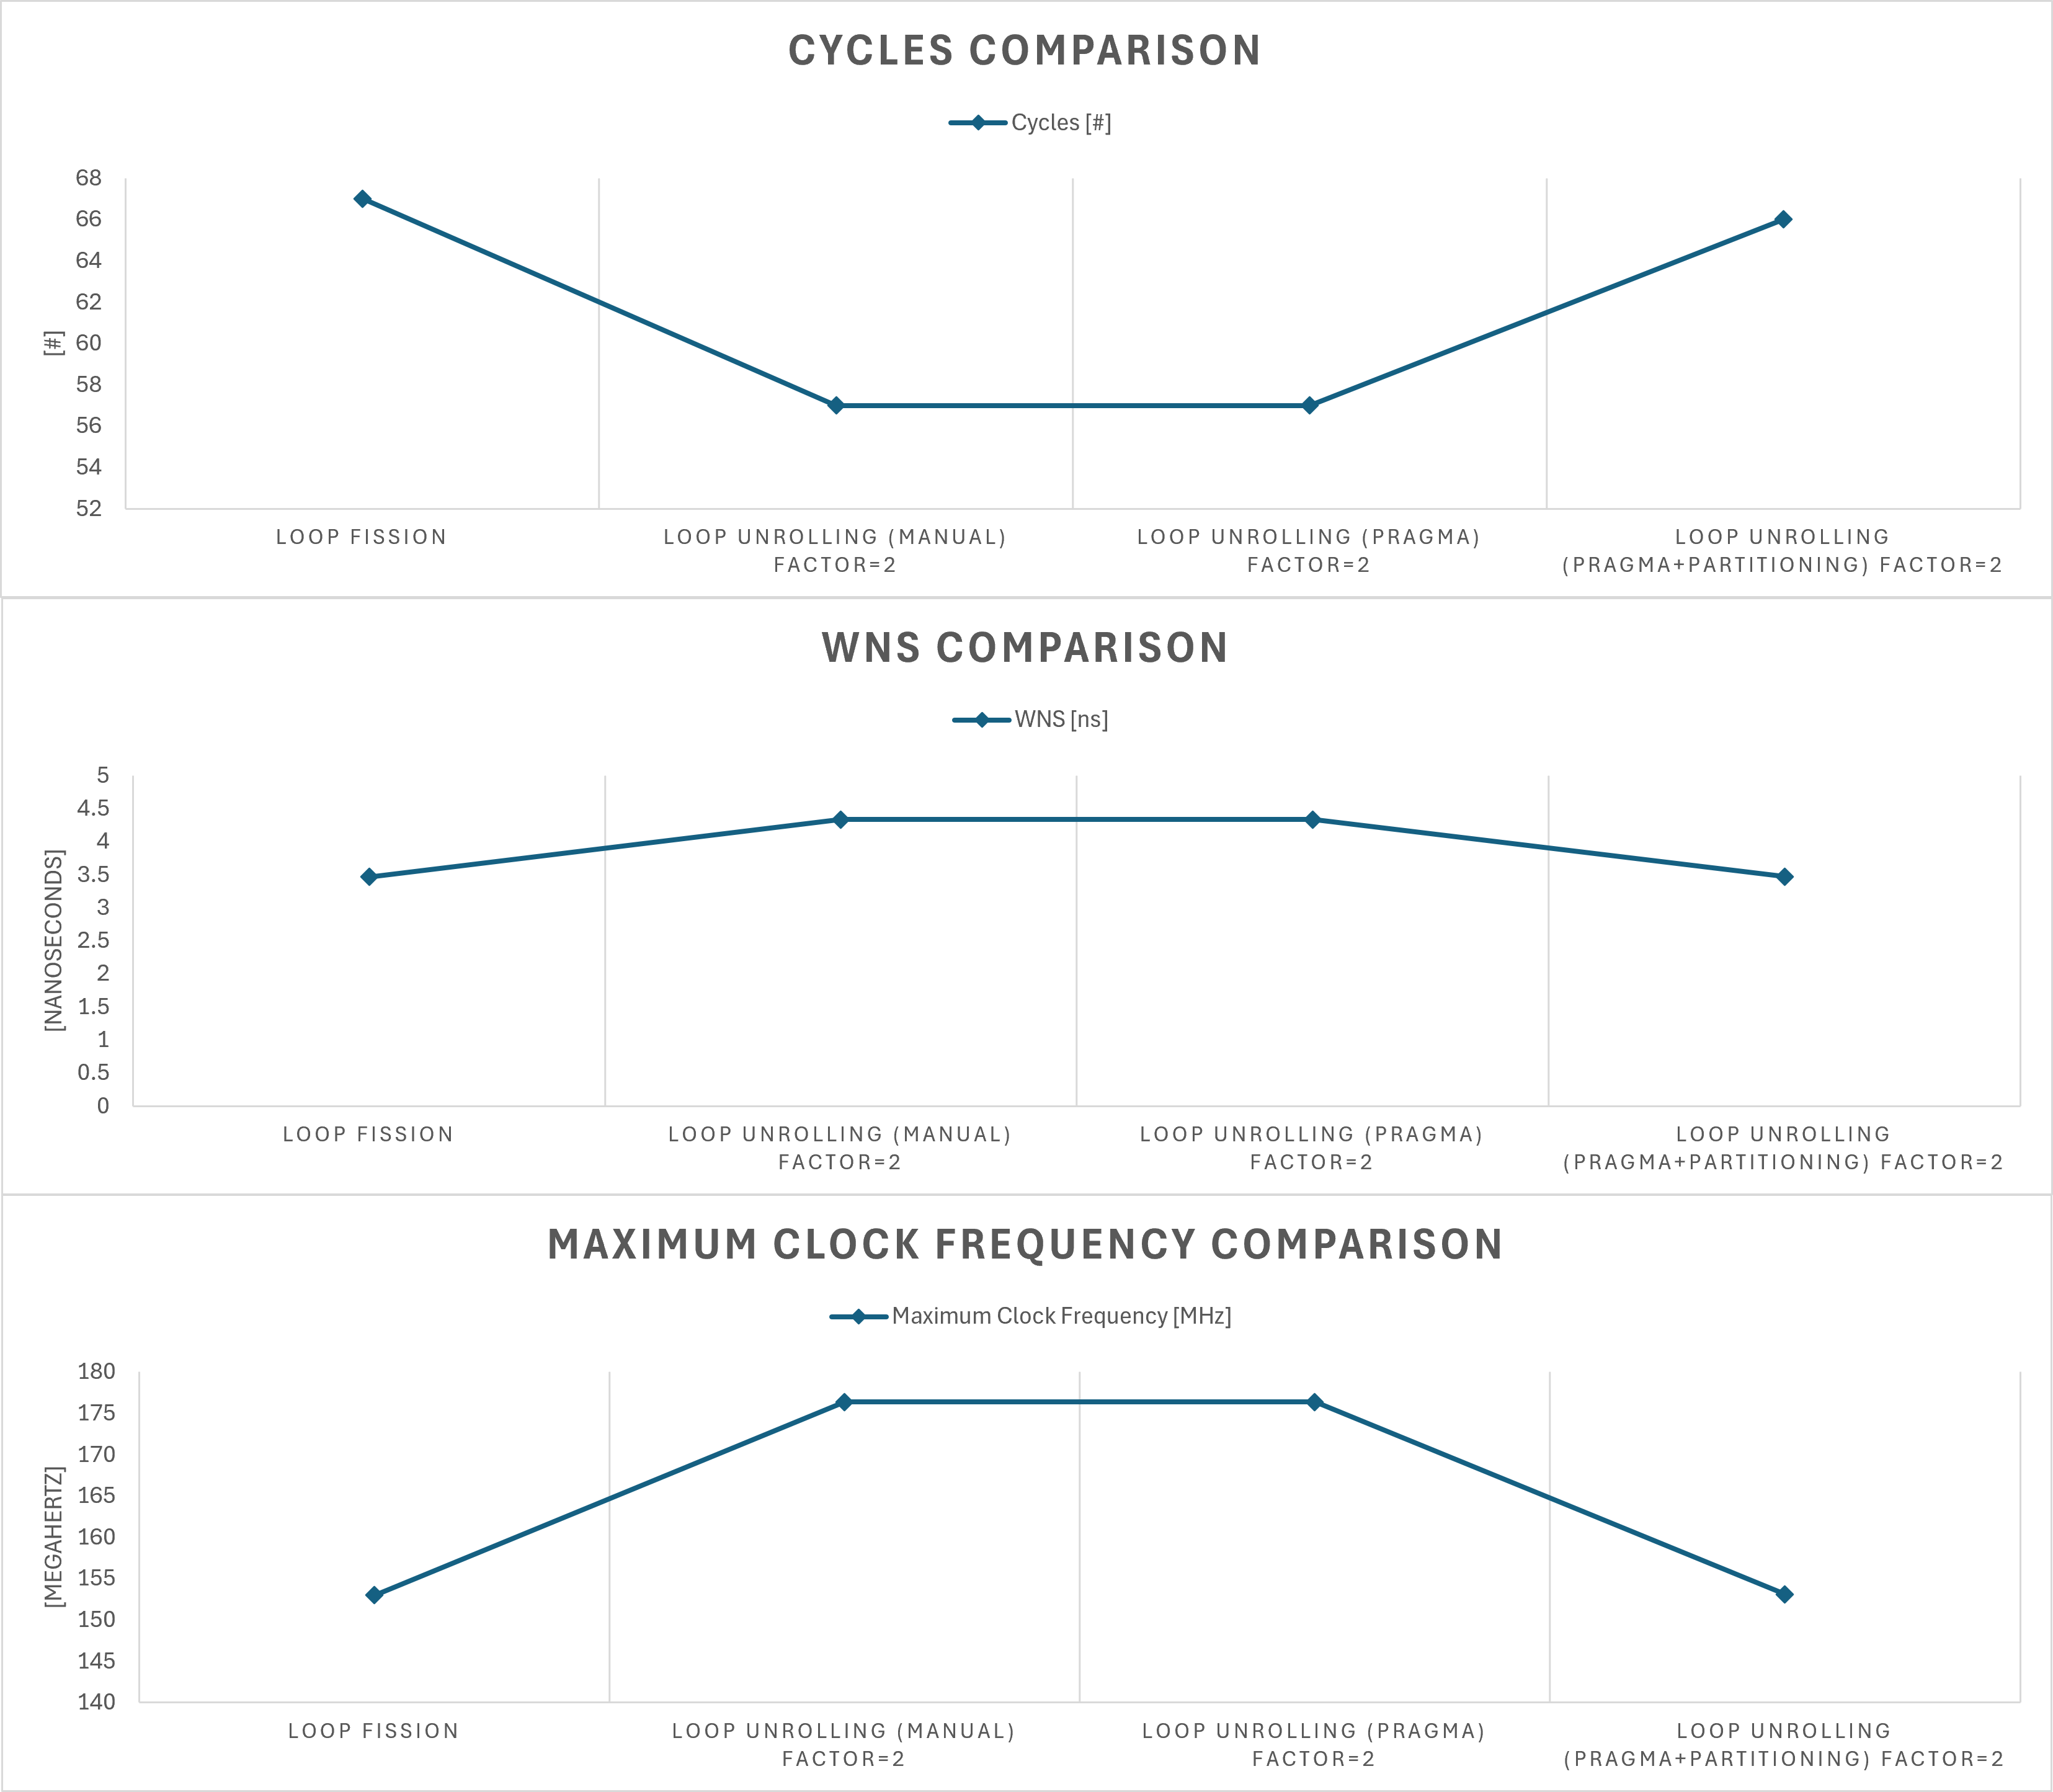
\includegraphics[width=0.8\textwidth]{solutions/loop_unrolling/factor2/loopunrollingfactor2timing.png}
    \caption{Vivado Loop Unrolling Factor=2 Timing Plot}
    \label{fig:vivado-loop-unrolling-factor2-solution-timing-plot}
\end{figure}

Per quanto riguarda, invece, la potenza dinamica associata alle tre soluzioni hardware proposte in questa sezione, è possibile notare come i contributi associati al Clock Enable e Clocks risultano essere notevolmente più grandi in corrispondenza dell'implementazione basata su partizionamento. Questo potrebbe essere causato dal notevole aumento dell'utilizzazione dei FF per questa solution. 

\begin{table}[H]
    \centering
    \begin{tabular}{|c|c|c|c|c|c|c|c|}
        \hline
        \textbf{Solution} & \textbf{BRAM} & \textbf{Clock} & \textbf{Clocks} & \textbf{DSP} & \textbf{Logic} & \textbf{Set/}& \textbf{Data} \\
        & & \textbf{Enable} & & & & \textbf{Reset} & \\
        \hline
        Manuale & 1.250551548 & 0.096387172 & 0.900532817 & 0.268251897 & 0.260709843 & 0.003146866 & 0.423992984 \\
        \hline
        Automatico & 1.240851358 & 0.082524632 & 0.960682868 & 0.272355421 & 0.266662013 & 0.00428147 & 0.425589533 \\
        \hline
        Automatico & & & & & & & \\
        con & 0 & 0.325270201 & 2.352835611 & 0.263715046 & 0.575191109 & 0.007010513 & 0.750690058 \\
        Partitioning & & & & & & & \\
        \hline
    \end{tabular}
    \caption{Vivado Loop Unrolling Factor=2 Solution Dynamic Power Report [mW]}
    \label{tab:vivado-loop-unrolling-factor2-solution-dynamic-power-reproot}
\end{table}

Infatti, è possibile riscontrare un aumento della potenza dinamica totale e dell'energia per singola operazione in corrispondenza dell'architettura basata su unrolling e partitioning. Invece, per quanto riguarda le altre due solution (unrolling manuale e automatico), entrambi i parametri appena citati risultano essere i medesimi. 

\begin{table}[H]
    \centering
    \begin{minipage}[t]{0.45\linewidth}
        \centering
        \begin{tabular}{|c|c|}
            \hline
            \textbf{Solution} & \textbf{Dynamic Total} \\
            \hline
            Manuale & 3.203573127 \\
            \hline
            Automatico & 3.252947294 \\
            \hline
            Automatico & 4.274712538 \\
            con Partitioning & \\
            \hline
        \end{tabular}
        \caption{Vivado Loop Unrolling Factor=2 Solution Dynamic Power Report [mW]}
        \label{tab:vivado-loop-unrolling-factor2-solution-dynamic-power-reproot}
    \end{minipage}
    \hfill
    \centering
    \begin{minipage}[t]{0.45\linewidth}
        \centering
        \begin{tabular}{|c|c|}
            \hline
            \textbf{Solution} & \textbf{Energy Single Operation} \\
            \hline
            Manuale & 32.03573127 \\
            \hline
            Automatico & 32.52947294 \\
            \hline
            Automatico & 42.74712538 \\
            con Partitioning & \\
            \hline
        \end{tabular}
        \caption{Vivado Loop Unrolling Factor=2 Solution Energy Single Operation Report [pJ]}
        \label{tab:vivado-loop-unrolling-factor2-solution-solution-energy-single-operation-reproot}
    \end{minipage}
\end{table}

Analizzando graficamente queste tre soluzioni e in aggiunta anche l'implementazione basata sulla scissione del loop, è possibile notare come quella basasta su loop fission presenta un medesimo valore di potenza dinamica totale ed energia per singola operazione rispetto alle due soluzioni di unrolling manuale e automatico.

\begin{figure}[H]
    \centering
    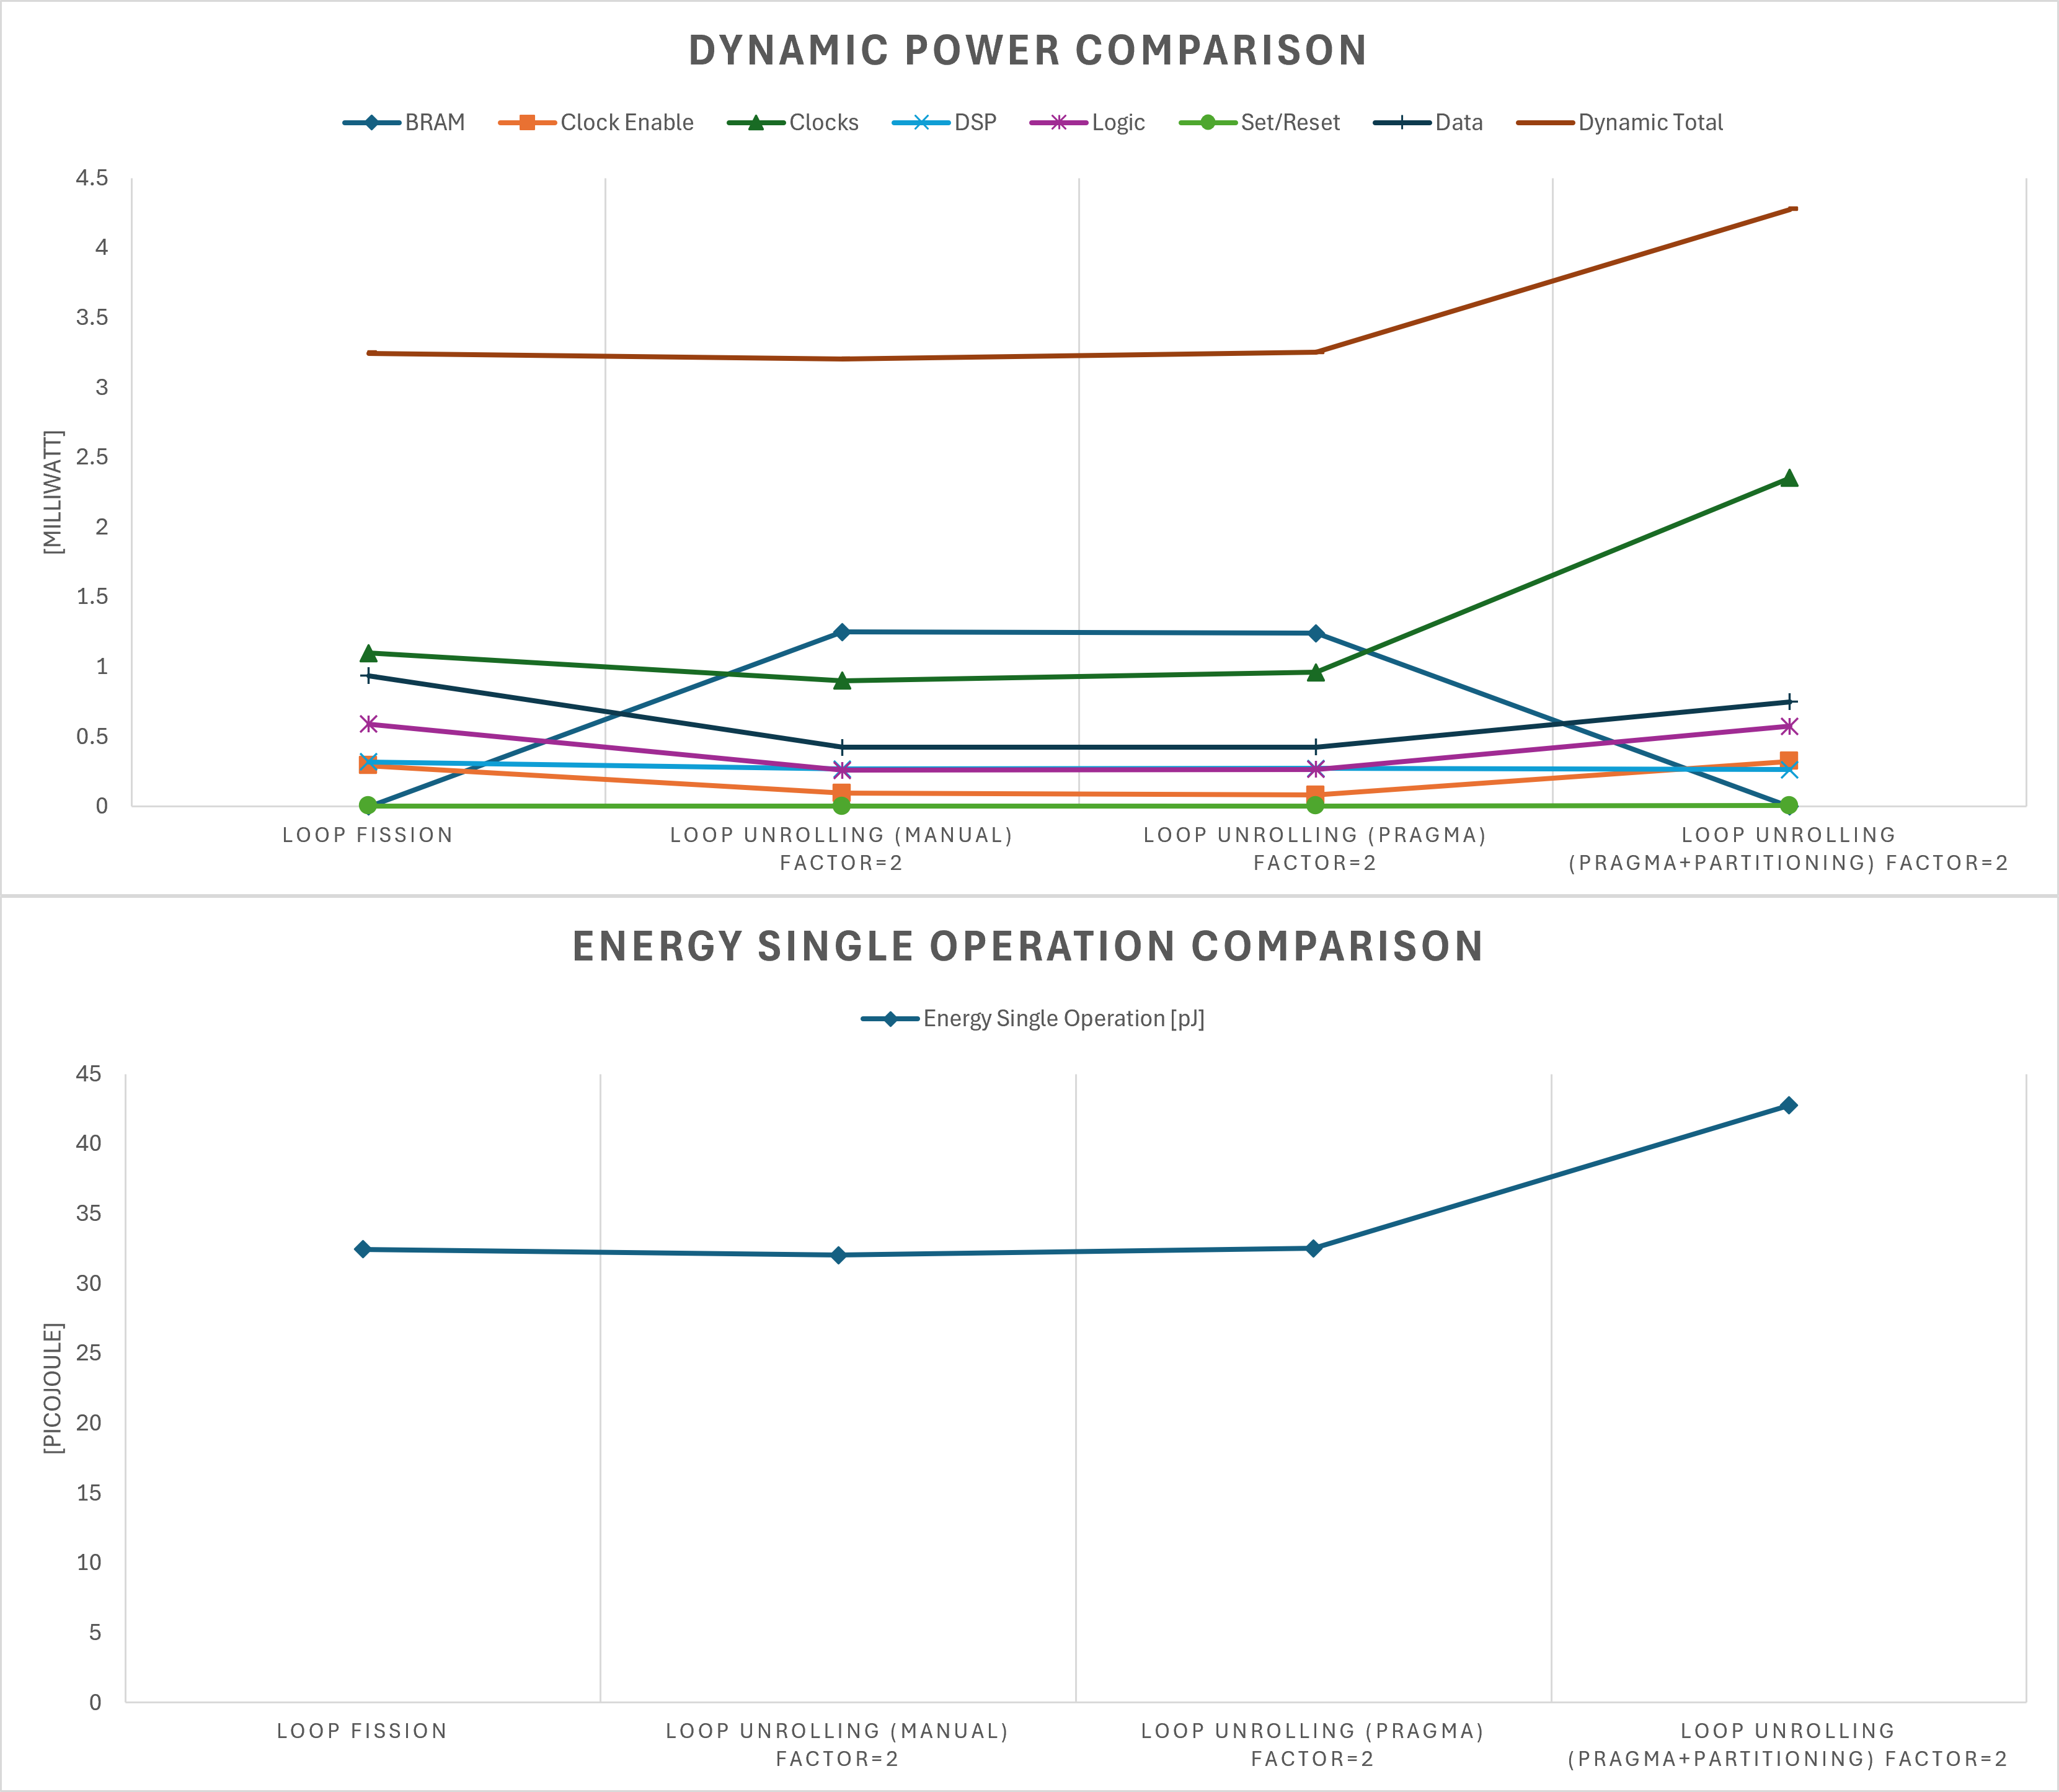
\includegraphics[width=\textwidth]{solutions/loop_unrolling/factor2/loopunrollingfactor2power.png}
    \caption{Vivado Loop Unrolling Factor=2 Dynamic Power Plot}
    \label{fig:vivado-loop-unrolling-factor2-solution-power-plot}
\end{figure}